\documentclass[aspectratio=169,11pt]{beamer}

\def\courseTitle{Industrial Security (Bachelor)}
\def\courseSubtitle{Section 06 -- Vulnerabilities and Assessment}
\def\sectionNumber{06}
\def\sectionTitle{Vulnerabilities and Assessment}

% =====================================================================
% Industrial Security lecture series -- modern Beamer preamble.
%
% Each slide deck must define the following BEFORE \input{}-ing this:
%   \def\courseTitle{...}        e.g. Industrial Security (Bachelor)
%   \def\courseSubtitle{...}     e.g. Section 3 -- Network Architecture
%   \def\sectionNumber{...}      e.g. 03
%   \def\sectionTitle{...}       e.g. Industrial Network Architectures
%
% Optional:
%   \def\courseAuthor{...}       defaults to "Lecture Notes"
%   \def\courseInstitute{...}    defaults to "Department of Computer Science"
%   \def\companyLogo{...}        path to a logo image (PDF/PNG/JPG).
%
% Callout macros (use anywhere inside a frame):
%   \begin{notebox}{title}      ... \end{notebox}
%   \begin{importantbox}{title} ... \end{importantbox}
%   \begin{warningbox}{title}   ... \end{warningbox}
%   \begin{tipbox}{title}       ... \end{tipbox}
%   \begin{defbox}{title}       ... \end{defbox}
%   \begin{takeawaybox}{title}  ... \end{takeawaybox}
%   \begin{quotebox}            ... \end{quotebox}
% =====================================================================

% --- Speaker-notes mode (toggled by Makefile via -usepretex) ----------
% When notesmode=1, build a side-by-side slide+notes PDF for the
% lecturer. When unset/0, build the clean slides-only PDF.
\providecommand{\notesmode}{0}
\ifnum\notesmode=1
  \usepackage{pgfpages}
  \setbeameroption{show notes on second screen=right}
  \setbeamerfont{note page}{size=\small}
\fi

\usepackage[utf8]{inputenc}
\usepackage[T1]{fontenc}
\usepackage[english]{babel}
% Modern type pair: IBM Plex Sans for text, IBM Plex Mono for code.
% Math stays in lmodern; Plex is the dominant family on every text frame.
\usepackage{plex-sans}
\usepackage{plex-mono}
\renewcommand{\familydefault}{\sfdefault}
\usepackage[activate={true,nocompatibility},final,tracking=true,kerning=true,spacing=true,factor=1100,stretch=10,shrink=10]{microtype}
\usepackage{graphicx}
\usepackage{listings}
\usepackage{xcolor}
\usepackage{colortbl}
\usepackage{tikz}
\usepackage{booktabs}
\usepackage{array}
\usepackage{hyperref}
\usepackage{amsmath}
\usepackage{amssymb}
\usepackage{tcolorbox}
\tcbuselibrary{skins, breakable, raster}
\usepackage{fontawesome5}

% =====================================================================
% Shared TikZ styles for the Industrial Security lecture series.
% Loaded by every slide deck and exercise sheet that uses TikZ.
% =====================================================================

\usetikzlibrary{
  arrows.meta,
  shapes,
  shapes.geometric,
  shapes.symbols,
  shapes.multipart,
  positioning,
  fit,
  calc,
  backgrounds,
  decorations.pathmorphing,
  decorations.pathreplacing,
  decorations.text,
  patterns,
  matrix,
  shadows
}

% --- colour palette --------------------------------------------------
\definecolor{isOT}{HTML}{1F4E79}     % OT (deep blue)
\definecolor{isIT}{HTML}{6F2DA8}     % IT (purple)
\definecolor{isSafety}{HTML}{C00000} % safety red
\definecolor{isNet}{HTML}{2E7D32}    % network green
\definecolor{isAttack}{HTML}{B23A48} % attack red
\definecolor{isAccent}{HTML}{E08E0B} % amber
\definecolor{isMute}{HTML}{6B6B6B}   % grey
\definecolor{isLight}{HTML}{EDF2F8}  % light background
\definecolor{isPLC}{HTML}{2C5282}
\definecolor{isHMI}{HTML}{2F855A}
\definecolor{isSCADA}{HTML}{6B46C1}

% --- generic node styles --------------------------------------------
\tikzset{
  isnode/.style={
    draw, rounded corners=2pt, minimum height=8mm, minimum width=18mm,
    font=\small, align=center, thick
  },
  isbox/.style={isnode, fill=isLight},
  plc/.style={isnode, fill=isPLC!15, draw=isPLC, thick},
  hmi/.style={isnode, fill=isHMI!15, draw=isHMI, thick},
  scada/.style={isnode, fill=isSCADA!15, draw=isSCADA, thick},
  sensor/.style={isnode, fill=isNet!10, draw=isNet, minimum height=6mm, minimum width=14mm, font=\scriptsize},
  actuator/.style={isnode, fill=isAccent!15, draw=isAccent, minimum height=6mm, minimum width=14mm, font=\scriptsize},
  firewall/.style={isnode, fill=isAttack!15, draw=isAttack, thick},
  server/.style={isnode, fill=isMute!15, draw=isMute!80, thick},
  switch/.style={isnode, fill=isLight, draw=black!60, minimum height=6mm, minimum width=14mm, font=\scriptsize},
  workstation/.style={isnode, fill=white, draw=isOT, thick},
  attacker/.style={isnode, fill=isAttack!20, draw=isAttack, thick, font=\small\bfseries},
  inetnode/.style={draw, ellipse, minimum width=24mm, minimum height=10mm, font=\scriptsize, fill=isLight, thick},
  process/.style={isnode, fill=isOT!15, draw=isOT, thick, minimum width=24mm},
  zone/.style={
    draw, rounded corners=4pt, thick, dashed, inner sep=4mm
  },
  conduit/.style={-{Stealth[length=2.5mm]}, thick, isNet!80!black},
  attack/.style={-{Stealth[length=2.5mm]}, thick, isAttack, dashed},
  flow/.style={-{Stealth[length=2.5mm]}, thick, isOT!70!black},
  netline/.style={thick, black!60},
  axisline/.style={-{Stealth[length=2mm]}, thick, black!70},
  tag/.style={font=\scriptsize\itshape, fill=white, inner sep=1pt},
  level/.style={
    draw, fill=isLight, minimum width=0.85\linewidth, minimum height=8mm,
    font=\small, anchor=west
  },
  brace/.style={decorate, decoration={brace, amplitude=4pt, raise=2pt}},
  legendbox/.style={draw, rounded corners=2pt, fill=isLight, inner sep=2mm, font=\scriptsize, align=left}
}

% --- handy macros ----------------------------------------------------
% \plcicon, \hmiicon etc as simple labelled boxes; useful inline.
\newcommand{\plcicon}[1][PLC]{\tikz[baseline=-0.6ex]{\node[plc, minimum width=10mm, minimum height=5mm, font=\scriptsize, inner sep=1pt]{#1};}}
\newcommand{\hmiicon}[1][HMI]{\tikz[baseline=-0.6ex]{\node[hmi, minimum width=10mm, minimum height=5mm, font=\scriptsize, inner sep=1pt]{#1};}}
\newcommand{\fwicon}[1][FW]{\tikz[baseline=-0.6ex]{\node[firewall, minimum width=10mm, minimum height=5mm, font=\scriptsize, inner sep=1pt]{#1};}}


\graphicspath{{.}{../../../template/}}

% --- defaults --------------------------------------------------------
\providecommand{\courseAuthor}{Lecture Notes}
\providecommand{\courseInstitute}{Department of Computer Science}
\providecommand{\companyLogo}{logo}

% --- modern palette --------------------------------------------------
\definecolor{slideAccent}{HTML}{1F4E79}       % primary navy
\definecolor{slideSecondary}{HTML}{E08E0B}    % amber accent

% --- Corporate branding overrides ------------------------------------
% A user-editable `branding.tex` at the repo root can override the
% logo path, author/institute lines, and brand colours. If the file is
% missing the built-in defaults above stay in effect.
\IfFileExists{../../../branding.tex}{% =====================================================================
% Corporate / institutional branding -- single file to customise the
% look of the entire course (slides, notes, exercises, labs).
%
% HOW TO REBRAND IN UNDER A MINUTE:
%   1. Replace `branding/logo.pdf` with your own logo
%      (PDF preferred; PNG and JPG also work -- name it `logo.<ext>`).
%   2. (Optional) change the two colours below to your brand palette.
%   3. (Optional) override the author/institute lines below.
%   4. Re-run `make` at the repo root. That's it.
%
% Everything in this file has sensible defaults; you can delete a line
% to fall back to the built-in defaults, or comment it out.
%
% This file is loaded automatically by the slides, exercise, and lab
% preambles -- you never need to \input it manually.
% =====================================================================

% --- Logo --------------------------------------------------------------
% Path is resolved from each leaf-build directory; the default points at
% the shared `branding/` folder at the repo root. If you put your logo
% somewhere else, set the full or relative path here (without extension):
\renewcommand{\companyLogo}{../../../branding/logo}

% --- Author / institute (appears on the title page footer) ------------
\renewcommand{\courseAuthor}{}
\renewcommand{\courseInstitute}{}

% --- Brand colours ----------------------------------------------------
% slideAccent      = primary brand colour (title bands, accent rule)
% slideSecondary   = secondary brand colour (section badge, highlight)
% Both use HTML hex codes. Keep enough contrast against white text.
\definecolor{slideAccent}{HTML}{00205B}      % deep navy
\definecolor{slideSecondary}{HTML}{00A0DC}   % light blue accent
}{}
\definecolor{slideTitle}{HTML}{0F2A44}        % near-black navy
\definecolor{slideMuted}{HTML}{6B6B6B}
\definecolor{slideBg}{HTML}{FFFFFF}
\definecolor{slidePanel}{HTML}{F4F7FB}
\definecolor{slideRule}{HTML}{D6DEE8}

% Callout colours
\definecolor{calNote}{HTML}{1F4E79}
\definecolor{calImportant}{HTML}{B23A48}
\definecolor{calWarning}{HTML}{C77700}
\definecolor{calTip}{HTML}{2E7D32}
\definecolor{calDef}{HTML}{6B46C1}
\definecolor{calTake}{HTML}{0F2A44}

% --- beamer theme ---------------------------------------------------
\useinnertheme{rectangles}
\usefonttheme{professionalfonts}

\setbeamertemplate{navigation symbols}{}
\setbeamertemplate{itemize items}[circle]
\setbeamertemplate{enumerate items}[default]
\setbeamertemplate{section in toc}[ball numbered]
\setbeamercolor{section in toc}{fg=slideTitle}

% Colours
\setbeamercolor{normal text}{fg=slideTitle, bg=slideBg}
\setbeamercolor{title}{fg=slideAccent}
\setbeamercolor{subtitle}{fg=slideMuted}
\setbeamercolor{frametitle}{fg=slideAccent}
\setbeamercolor{structure}{fg=slideAccent}
\setbeamercolor{itemize item}{fg=slideAccent}
\setbeamercolor{itemize subitem}{fg=slideSecondary}
\setbeamercolor{block title}{fg=white, bg=slideAccent}
\setbeamercolor{block body}{fg=slideTitle, bg=slidePanel}
\setbeamercolor{alerted text}{fg=slideSecondary}

% Fonts
\setbeamerfont{title}{series=\bfseries, size=\Large}
\setbeamerfont{subtitle}{series=\mdseries, size=\normalsize}
\setbeamerfont{frametitle}{series=\bfseries, size=\large}
\setbeamerfont{block title}{series=\bfseries, size=\normalsize}
\setbeamerfont{footline}{size=\tiny}

% --- frametitle: title bar + accent underline + section badge -------
% The accent rules are wrapped in a zero-width box so they never
% contribute to the surrounding hbox width (no Overfull warnings).
\setbeamertemplate{frametitle}{%
  \nointerlineskip
  \begin{beamercolorbox}[wd=\paperwidth, ht=2.8ex, dp=1.6ex, leftskip=1.2em, rightskip=1.2em]{frametitle}%
    \usebeamerfont{frametitle}\insertframetitle%
    \hfill
    {\color{slideMuted}\small \sectionNumber}%
  \end{beamercolorbox}%
  \nointerlineskip
  \makebox[0pt][l]{\hspace*{1.2em}\textcolor{slideSecondary}{\rule{2.5em}{1pt}}\textcolor{slideAccent}{\rule{\dimexpr\paperwidth-3.7em\relax}{1pt}}}%
  \par\vskip4pt
}

% --- footer ---------------------------------------------------------
\defbeamertemplate*{footline}{is-footer}{%
  \leavevmode%
  \hbox{%
    \begin{beamercolorbox}[wd=.55\paperwidth, ht=2.4ex, dp=1ex, leftskip=1em]{author in head/foot}%
      {\color{slideMuted}\tiny \courseTitle{} \;\; $\bullet$ \;\; Section \sectionNumber{} -- \sectionTitle}%
    \end{beamercolorbox}%
    \begin{beamercolorbox}[wd=.45\paperwidth, ht=2.4ex, dp=1ex, rightskip=1em]{title in head/foot}%
      \hfill {\color{slideMuted}\tiny \insertframenumber{} / \inserttotalframenumber}%
    \end{beamercolorbox}%
  }%
  \vskip2pt
}

% --- listings -------------------------------------------------------
\definecolor{codebg}{HTML}{F4F7FB}
\definecolor{codekw}{HTML}{0F2A44}
\definecolor{codestr}{HTML}{8B3A3A}
\definecolor{codecom}{HTML}{5A7D54}

\lstset{
    backgroundcolor=\color{codebg},
    basicstyle=\ttfamily\scriptsize\color{slideTitle},
    keywordstyle=\color{codekw}\bfseries,
    stringstyle=\color{codestr},
    commentstyle=\color{codecom}\itshape,
    breaklines=true,
    frame=leftline,
    framerule=2pt,
    rulecolor=\color{slideAccent},
    numbers=left,
    numberstyle=\tiny\color{slideMuted},
    numbersep=8pt,
    showstringspaces=false,
    tabsize=2,
    captionpos=b,
    xleftmargin=0.6em
}

% --- callout boxes --------------------------------------------------
% Shared base style for all callout boxes.
% Subtle drop shadow gives the boxes a hint of elevation without distraction.
\tcbset{
  isCallout/.style={
    enhanced, breakable, sharp corners=northeast,
    arc=2pt, boxrule=0pt,
    leftrule=3pt,
    fonttitle=\bfseries\small,
    coltitle=white,
    fontupper=\small,
    left=2mm, right=2mm, top=1.5mm, bottom=1.5mm,
    drop fuzzy shadow=black!30,
    title={#1}
  }
}

\newtcolorbox{notebox}[1]{
  isCallout={#1},
  colback=calNote!8, colframe=calNote, leftrule=3pt,
  colbacktitle=calNote, attach boxed title to top left={xshift=2mm, yshift=-1.2mm},
  boxed title style={colback=calNote, arc=1pt, boxrule=0pt, left=2mm, right=2mm, top=0.5mm, bottom=0.5mm}
}

\newtcolorbox{importantbox}[1]{
  isCallout={#1},
  colback=calImportant!7, colframe=calImportant, leftrule=4pt,
  colbacktitle=calImportant, attach boxed title to top left={xshift=2mm, yshift=-1.2mm},
  boxed title style={colback=calImportant, arc=1pt, boxrule=0pt, left=2mm, right=2mm, top=0.5mm, bottom=0.5mm}
}

\newtcolorbox{warningbox}[1]{
  isCallout={#1},
  colback=calWarning!10, colframe=calWarning, leftrule=4pt,
  colbacktitle=calWarning, attach boxed title to top left={xshift=2mm, yshift=-1.2mm},
  boxed title style={colback=calWarning, arc=1pt, boxrule=0pt, left=2mm, right=2mm, top=0.5mm, bottom=0.5mm}
}

% Alias warnbox = warningbox, with an optional title (default = "Caution")
\newtcolorbox{warnbox}[1][Caution]{
  isCallout={#1},
  colback=calWarning!10, colframe=calWarning, leftrule=4pt,
  colbacktitle=calWarning, attach boxed title to top left={xshift=2mm, yshift=-1.2mm},
  boxed title style={colback=calWarning, arc=1pt, boxrule=0pt, left=2mm, right=2mm, top=0.5mm, bottom=0.5mm}
}

\newtcolorbox{tipbox}[1]{
  isCallout={#1},
  colback=calTip!8, colframe=calTip, leftrule=3pt,
  colbacktitle=calTip, attach boxed title to top left={xshift=2mm, yshift=-1.2mm},
  boxed title style={colback=calTip, arc=1pt, boxrule=0pt, left=2mm, right=2mm, top=0.5mm, bottom=0.5mm}
}

\newtcolorbox{defbox}[1]{
  isCallout={#1},
  colback=calDef!8, colframe=calDef, leftrule=3pt,
  colbacktitle=calDef, attach boxed title to top left={xshift=2mm, yshift=-1.2mm},
  boxed title style={colback=calDef, arc=1pt, boxrule=0pt, left=2mm, right=2mm, top=0.5mm, bottom=0.5mm}
}

\newtcolorbox{takeawaybox}[1]{
  enhanced, breakable, arc=3pt, boxrule=0pt,
  colback=calTake!7, colframe=calTake,
  toptitle=2mm, bottomtitle=2mm,
  fonttitle=\bfseries\normalsize, coltitle=white,
  colbacktitle=calTake,
  fontupper=\small,
  title={\faStar~Key Takeaway: #1},
  left=3mm, right=3mm, top=2mm, bottom=2mm
}

\newtcolorbox{quotebox}{
  enhanced, breakable, arc=2pt, boxrule=0pt,
  colback=slidePanel, colframe=slideMuted,
  leftrule=3pt, top=2mm, bottom=2mm, left=3mm, right=3mm,
  fontupper=\itshape\small,
}

% Convenience: inline highlight badge
\newcommand{\remembertag}{\tikz[baseline=-0.7ex]\node[fill=calImportant, text=white, font=\scriptsize\bfseries, rounded corners=2pt, inner sep=2pt]{REMEMBER};}
\newcommand{\tldr}{\tikz[baseline=-0.7ex]\node[fill=calTake, text=white, font=\scriptsize\bfseries, rounded corners=2pt, inner sep=2pt]{TL;DR};}

% Source attribution: tiny grey line, anchored bottom-left of the content area
% Usage:  \source{Symantec, \emph{W32.Stuxnet Dossier} v1.4, 2011.}
% Multiple sources:  \source{X.\ Y., 2018; Z, 2020.}
\newcommand{\source}[1]{%
  \par\nointerlineskip\vspace{0.4mm}%
  {\color{slideMuted}\fontsize{5.5}{6.5}\selectfont\textit{Source:} #1\par}%
}

% References slide: aggregate citations + further reading at the end of a section.
% Usage:  \referencesframe{ \item ... \item ... }
% The `frame` environment must be written literally in the deck, so this is a
% macro rather than a wrapper environment (beamer collects the frame body and
% trips over \newenvironment wrappers).
%
% allowframebreakstemplate=\insertcontinuationcount silences the trailing roman
% numeral when content fits on a single page.
\setbeamertemplate{frametitle continuation}[from second]
\newcommand{\referencesframe}[1]{%
  \begin{frame}[allowframebreaks]{References -- Section \sectionNumber}
    \fontsize{7.5}{9}\selectfont
    \setlength{\itemsep}{1pt}
    \begin{itemize}#1\end{itemize}
  \end{frame}%
}

% --- title page -----------------------------------------------------
\title[\courseTitle]{\courseTitle}
\subtitle{\courseSubtitle}
\author{\courseAuthor}
\institute{\courseInstitute}
\date{}

% Logo lookup: try the section directory, then the shared template/.
\newcommand{\showlogo}[1][2cm]{%
  \IfFileExists{\companyLogo.pdf}{\includegraphics[width=#1]{\companyLogo}}{%
    \IfFileExists{\companyLogo.png}{\includegraphics[width=#1]{\companyLogo}}{%
      \IfFileExists{\companyLogo.jpg}{\includegraphics[width=#1]{\companyLogo}}{%
        \IfFileExists{../../../template/\companyLogo.pdf}{\includegraphics[width=#1]{../../../template/\companyLogo}}{%
          \rule{0pt}{0pt}}}}}}

\setbeamertemplate{title page}{%
  
\begin{tikzpicture}[remember picture, overlay]
    % accent band (taller to fit wrapped titles)
    \fill[slideAccent] (current page.north west) rectangle ([yshift=-3.4cm]current page.north east);
    \fill[slideSecondary] ([yshift=-3.4cm]current page.north west) rectangle ([yshift=-3.55cm]current page.north east);
    % section badge
    \node[fill=slideSecondary, text=white, font=\bfseries\normalsize, rounded corners=3pt, inner sep=4pt, anchor=north west]
      at ([xshift=1.2cm, yshift=-0.7cm]current page.north west) {Section \sectionNumber};
    % Course title (wraps if long)
    \node[anchor=north west, text=white, font=\bfseries\Large, align=left, text width=11cm]
      at ([xshift=1.2cm, yshift=-1.5cm]current page.north west) {\courseTitle};
    % Subtitle (wraps; smaller, separated)
    \node[anchor=north west, text=white, font=\mdseries\small, align=left, text width=11cm]
      at ([xshift=1.2cm, yshift=-2.7cm]current page.north west) {\courseSubtitle};
    \node[anchor=north east] at ([xshift=-1.2cm, yshift=-1.0cm]current page.north east)
      {\showlogo[2cm]};
    \node[anchor=south west, text=slideMuted, font=\small, align=left, text width=11cm]
      at ([xshift=1.2cm, yshift=1.0cm]current page.south west)
      {\textbf{\sectionTitle}\\[2pt]\textit{\courseAuthor}\\{\scriptsize\courseInstitute}};
  \end{tikzpicture}
}

% --- helper macros --------------------------------------------------
\newcommand{\learningobjectives}[1]{%
  \begin{frame}{Learning Objectives}
    \begin{tipbox}{\faGraduationCap~By the end of this section you will be able to}
      \begin{itemize}\setlength{\itemsep}{2pt}#1\end{itemize}
    \end{tipbox}
  \end{frame}}

\newcommand{\sectionoverviewframe}{%
  \begin{frame}[plain,noframenumbering]
    \titlepage
  \end{frame}
  \begin{frame}{Outline -- Section \sectionNumber}
    \tableofcontents
  \end{frame}}

\AtBeginSection[]{%
  \begin{frame}[plain,noframenumbering]
    \begin{tikzpicture}[remember picture, overlay]
      \fill[slideAccent] (current page.north west) rectangle (current page.south east);
      \fill[slideSecondary] ([yshift=-1pt]current page.center -| current page.west)
                            rectangle ([yshift=1pt]current page.center -| current page.east);
      \node[text=white, font=\scriptsize, anchor=south west]
        at ([xshift=1.2cm, yshift=1.0cm]current page.south west)
        {Section \sectionNumber{} -- \sectionTitle};
      \node[text=slideSecondary, font=\bfseries\Huge, anchor=south]
        at ([yshift=0.4cm]current page.center)
        {\thesection};
      \node[text=white, font=\bfseries\LARGE, align=center, anchor=north, text width=12cm]
        at ([yshift=-0.6cm]current page.center)
        {\insertsection};
    \end{tikzpicture}
  \end{frame}}

\newcommand{\closingframe}{%
  \begin{frame}[plain,noframenumbering]
    \begin{tikzpicture}[remember picture, overlay]
      \fill[slideAccent] (current page.north west) rectangle (current page.south east);
      \node[text=white, font=\bfseries\Huge, anchor=center, align=center, text width=14cm]
        at ([yshift=8mm]current page.center) {End of Section \sectionNumber};
      \fill[slideSecondary] ([xshift=-1.5cm, yshift=-4mm]current page.center)
                            rectangle ([xshift=1.5cm, yshift=-6mm]current page.center);
      \node[text=white, font=\large, anchor=north, align=center, text width=14cm]
        at ([yshift=-1.2cm]current page.center) {\sectionTitle};
      \node[text=slideSecondary, font=\normalsize, anchor=south] at ([yshift=1.2cm]current page.south) {Questions and discussion};
      \node[anchor=south east] at ([xshift=-1cm, yshift=1cm]current page.south east) {\showlogo[1.5cm]};
    \end{tikzpicture}
  \end{frame}}


\begin{document}

\sectionoverviewframe

\learningobjectives{
  \item Find and interpret ICS vulnerability advisories.
  \item Apply CVSS v3.1 with environmental modifiers in an OT context.
  \item Plan a safe asset inventory across passive and active methods.
  \item Run a vulnerability management workflow that fits OT constraints.
}

\section{Vulnerability Intelligence}

\begin{frame}{Sources of ICS Vulnerability Intelligence}
\centering
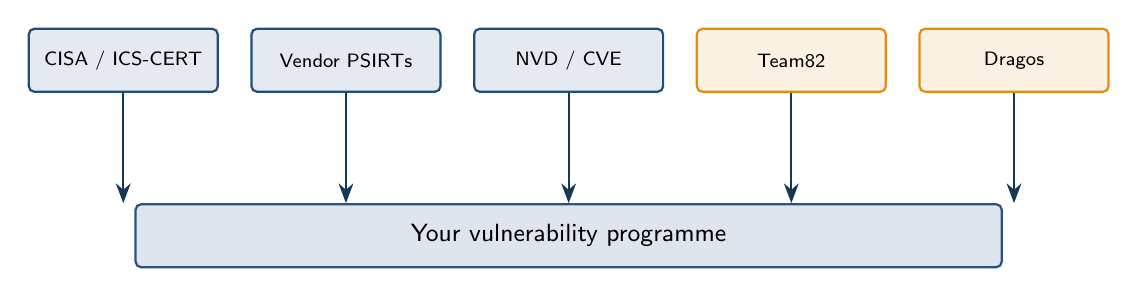
\begin{tikzpicture}[node distance=4mm]
  \node[server, fill=isOT!12, draw=isOT, minimum width=24mm, font=\scriptsize] (cisa) {CISA / ICS-CERT};
  \node[server, fill=isOT!12, draw=isOT, minimum width=24mm, font=\scriptsize, right=of cisa] (psirt) {Vendor PSIRTs};
  \node[server, fill=isOT!12, draw=isOT, minimum width=24mm, font=\scriptsize, right=of psirt] (nvd) {NVD / CVE};
  \node[server, fill=isAccent!12, draw=isAccent, minimum width=24mm, font=\scriptsize, right=of nvd] (claroty) {Team82};
  \node[server, fill=isAccent!12, draw=isAccent, minimum width=24mm, font=\scriptsize, right=of claroty] (dragos) {Dragos};
  \node[isbox, fill=isPLC!15, draw=isPLC, minimum width=110mm, below=14mm of {$(cisa.south)!0.5!(dragos.south)$}, font=\small] (you) {Your vulnerability programme};
  \foreach \n in {cisa,psirt,nvd,claroty,dragos}{\draw[flow] (\n.south) -- (\n.south |- you.north);}
\end{tikzpicture}
\note{
  Walk the room through the feed landscape: CISA ICSA advisories are the single most useful free feed, but they trail the vendor PSIRTs by weeks. Stress that nobody can rely on one source --- Team82 (Claroty), Dragos, Nozomi Labs, and Forescout Vedere Labs all surface bugs that never make it into NVD on the day of disclosure. Make the point that a vulnerability programme is a \emph{pipeline}, not a website you visit when you remember. Ask students which of these feeds they think publishes the most ICS-specific content per year, then reveal that CISA and the vendor PSIRTs together dwarf NVD for OT relevance.
}
\end{frame}

\begin{frame}{Anatomy of a CVE Advisory}
\centering
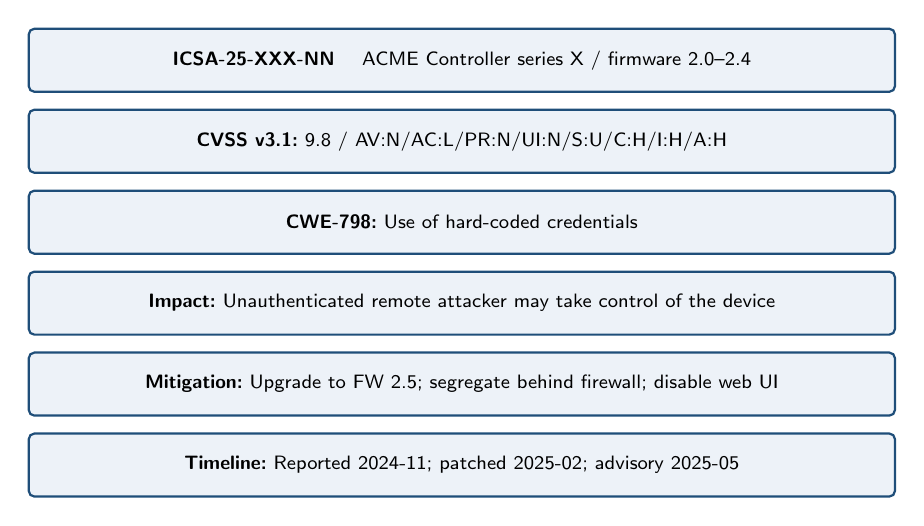
\begin{tikzpicture}[node distance=2mm]
  \node[isbox, fill=isLight, draw=isOT, minimum width=110mm, align=left, font=\scriptsize] (a)
    {\textbf{ICSA-25-XXX-NN} \quad ACME Controller series X / firmware 2.0--2.4};
  \node[isbox, fill=isLight, draw=isOT, minimum width=110mm, align=left, font=\scriptsize, below=of a] (b)
    {\textbf{CVSS v3.1:} 9.8 / AV:N/AC:L/PR:N/UI:N/S:U/C:H/I:H/A:H};
  \node[isbox, fill=isLight, draw=isOT, minimum width=110mm, align=left, font=\scriptsize, below=of b] (c)
    {\textbf{CWE-798:} Use of hard-coded credentials};
  \node[isbox, fill=isLight, draw=isOT, minimum width=110mm, align=left, font=\scriptsize, below=of c] (d)
    {\textbf{Impact:} Unauthenticated remote attacker may take control of the device};
  \node[isbox, fill=isLight, draw=isOT, minimum width=110mm, align=left, font=\scriptsize, below=of d] (e)
    {\textbf{Mitigation:} Upgrade to FW 2.5; segregate behind firewall; disable web UI};
  \node[isbox, fill=isLight, draw=isOT, minimum width=110mm, align=left, font=\scriptsize, below=of e] (f)
    {\textbf{Timeline:} Reported 2024-11; patched 2025-02; advisory 2025-05};
\end{tikzpicture}
\note{
  Walk the advisory top-to-bottom and explain each field --- the ICSA-ID encodes year and day-of-year, the affected firmware band is what the asset inventory must match against, and the CVSS vector is more informative than the headline score. Highlight the six-month gap between report and advisory --- that is normal in OT and explains why threat intel beats public feeds. Note that CWE-798 (hard-coded credentials) is the single most common root cause across PLCs in the last decade. Ask the TA to have students open a real CISA advisory on the lab laptops and read the same fields aloud --- it makes the structure stick.
}
\end{frame}

\begin{frame}{CVSS for ICS -- Caveats}
\centering
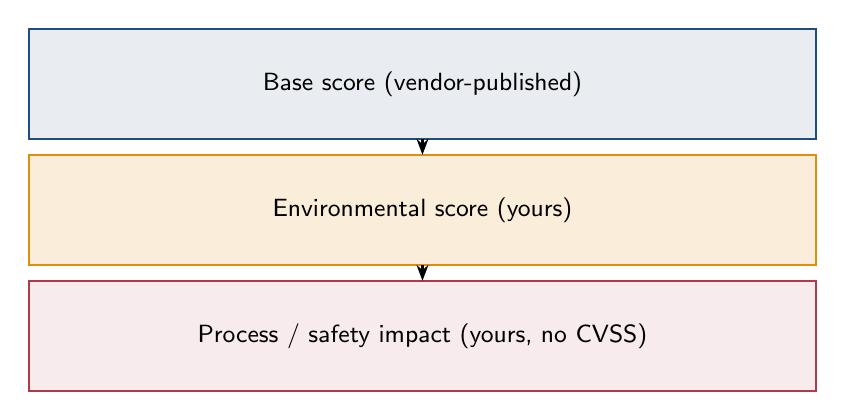
\begin{tikzpicture}
  \draw[fill=isOT!10, draw=isOT, thick] (0,0) rectangle (10,1.4) node[midway, font=\small]{Base score (vendor-published)};
  \draw[fill=isAccent!15, draw=isAccent, thick] (0,-1.6) rectangle (10,-0.2) node[midway, font=\small]{Environmental score (yours)};
  \draw[fill=isAttack!10, draw=isAttack, thick] (0,-3.2) rectangle (10,-1.8) node[midway, font=\small]{Process / safety impact (yours, no CVSS)};
  \draw[-{Stealth[length=2mm]}, thick] (5,0) -- (5,-0.2);
  \draw[-{Stealth[length=2mm]}, thick] (5,-1.6) -- (5,-1.8);
\end{tikzpicture}
\par\vspace{1mm}
{\footnotesize Base alone is misleading. ``Low Availability'' in IT may equal \emph{plant shutdown} in OT. Always combine with process consequence.}
\source{FIRST, \emph{CVSS v3.1 Specification Document}, 2019.}
\note{
  Show CVSS in its honest light: a base score of 9.8 on a PLC behind a one-way data diode is a different risk from the same 9.8 on a perimeter HMI. CISA started publishing environmental guidance for ICS because of exactly this issue. Pre-empt the IT mindset that a high CVSS means immediate patching --- in OT, patching is a project, not a sprint. The third row is the one CVSS does not capture at all: a low-availability bug that drops a safety interlock is plant-stop territory, not a ticket. Ask the room: if a vendor releases a critical patch but the next maintenance window is in six months, what compensating controls would they propose?
}
\end{frame}

\section{Asset Inventory and Scanning}

\begin{frame}{Asset Inventory -- The Foundation}
\centering
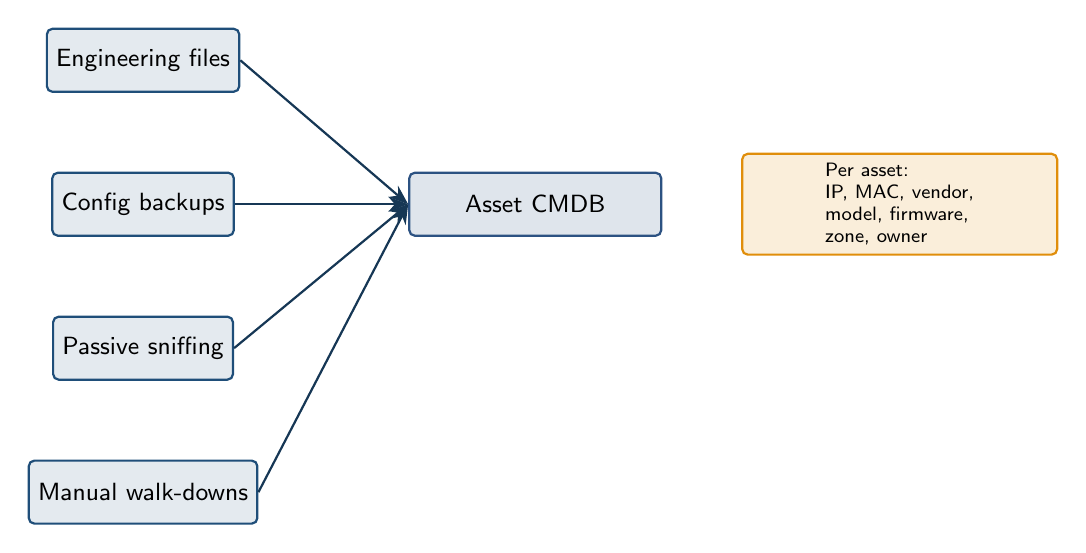
\begin{tikzpicture}[node distance=10mm]
  \node[isbox, fill=isOT!12, draw=isOT] (eng) {Engineering files};
  \node[isbox, fill=isOT!12, draw=isOT, below=of eng] (cfg) {Config backups};
  \node[isbox, fill=isOT!12, draw=isOT, below=of cfg] (pass) {Passive sniffing};
  \node[isbox, fill=isOT!12, draw=isOT, below=of pass] (walk) {Manual walk-downs};
  \node[server, right=22mm of cfg, fill=isPLC!15, draw=isPLC, minimum width=32mm] (cmdb) {Asset CMDB};
  \node[isbox, fill=isAccent!15, draw=isAccent, right=of cmdb, font=\scriptsize, align=left, minimum width=40mm]
    {Per asset:\\IP, MAC, vendor,\\model, firmware,\\zone, owner};
  \foreach \n in {eng,cfg,pass,walk}{\draw[flow] (\n.east) -- (cmdb.west);}
\end{tikzpicture}
\par\vspace{2mm}
\footnotesize ``You can't protect what you don't know you have.'' Firmware version is required to match CVEs.
\note{
  Drive home that everything downstream --- CVE matching, segmentation, incident response --- collapses without an accurate inventory. The dirty secret is that most plants discover 20--40\% more devices the first time they deploy a passive tool like Claroty CTD, Nozomi Guardian, or Microsoft Defender for IoT. Stress the four-input model on the slide: engineering files for what \emph{should} be there, config backups for ground truth, passive sniffing for what is actually talking, and walk-downs for the analogue gear that never appears on the wire. Firmware version is the load-bearing field --- without it you cannot answer ``are we affected?'' for any advisory. War story to share: a plant we visited had three undocumented Modbus gateways feeding a historian; passive scan found them in an afternoon.
}
\end{frame}

\begin{frame}{Passive vs.\ Active Scanning}
\centering
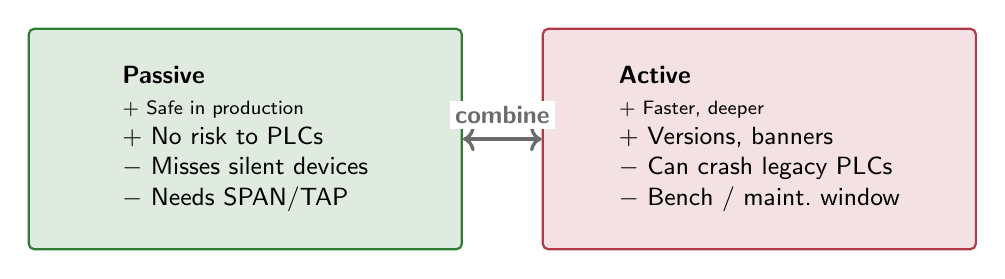
\begin{tikzpicture}[node distance=10mm]
  \node[isbox, fill=isNet!15, draw=isNet, minimum width=55mm, minimum height=28mm, align=left, font=\small]
    (p)
    {\textbf{Passive}\\\scriptsize
       $+$ Safe in production\\
       $+$ No risk to PLCs\\
       $-$ Misses silent devices\\
       $-$ Needs SPAN/TAP};
  \node[isbox, fill=isAttack!15, draw=isAttack, minimum width=55mm, minimum height=28mm, align=left, font=\small, right=of p]
    (a)
    {\textbf{Active}\\\scriptsize
       $+$ Faster, deeper\\
       $+$ Versions, banners\\
       $-$ Can crash legacy PLCs\\
       $-$ Bench / maint.\ window};
  \draw[<->, very thick, isMute] (p) -- node[above=3pt, font=\small\bfseries, fill=white, inner sep=2pt]{combine} (a);
\end{tikzpicture}
\note{
  Demolish the myth that ``passive is always safe'' --- it is mostly safe, but a misconfigured SPAN port can cause switch CPU spikes, and some passive tools do send the occasional active probe (read the manual). Tell the war story: a junior consultant ran an \texttt{nmap -sS} sweep against a live cement plant and bricked two 1990s-vintage PLCs that crashed on any unexpected TCP flag combination --- four-hour outage, vendor flew in, the consultant did not come back. The lesson is not ``never scan'' but ``never scan production without a documented bench result for that exact model.'' Tools like Tenable.ot, Forescout, and Armis advertise ``safe active'' modes but they still require vendor sign-off in regulated plants. Bridge to the next slide: even on a bench, you tune \texttt{nmap} to crawl, not sprint.
}
\end{frame}

\begin{frame}[fragile]{Safe \texttt{nmap} Against a Test PLC}
\centering
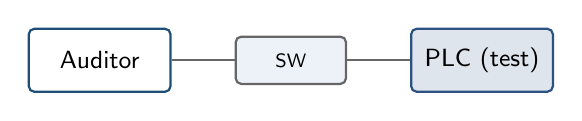
\begin{tikzpicture}[node distance=8mm]
  \node[workstation] (lap) {Auditor};
  \node[switch, right=of lap] (sw) {SW};
  \node[plc, right=of sw] (plc) {PLC (test)};
  \draw[netline] (lap) -- (sw); \draw[netline] (sw) -- (plc);
\end{tikzpicture}\par\vspace{3mm}
\begin{lstlisting}[basicstyle=\ttfamily\scriptsize, frame=single]
# Bench only -- never on production
nmap -sT -p 102,502,20000,44818,20256 \
     --max-rate 5 --scan-delay 200ms \
     -Pn 192.168.10.10

nmap -p 102 --script s7-info       192.168.10.10
nmap -p 502 --script modbus-discover 192.168.10.10
\end{lstlisting}
\note{
  Explain every flag: \texttt{-sT} avoids the half-open SYN scan that some legacy stacks mis-handle, \texttt{--max-rate 5} keeps the device from drowning, \texttt{--scan-delay 200ms} gives slow CPUs time to breathe, and \texttt{-Pn} skips the ICMP ping because many PLCs reply oddly. The port list covers the usual ICS suspects: 102 Siemens S7, 502 Modbus/TCP, 20000 DNP3, 44818 EtherNet/IP, 20256 PCWorx. Hammer home the comment on line one --- ``bench only.'' Even with these settings, the Nmap NSE scripts (\texttt{s7-info}, \texttt{modbus-discover}) send protocol-specific queries that can confuse some firmware versions. If a student asks ``can I try this at my internship?'', the answer is ``not without written approval and a tested rollback.''
}
\end{frame}

\section{Vulnerability Management Workflow}

\begin{frame}{Vulnerability Management Cycle}
\centering
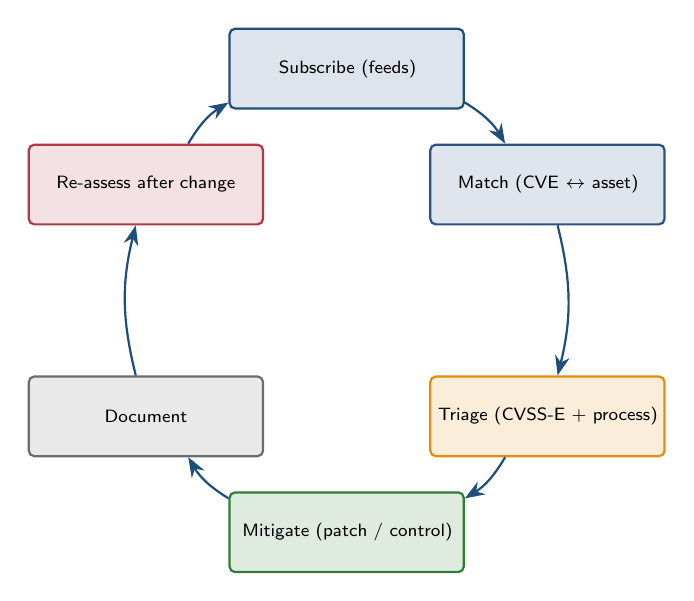
\begin{tikzpicture}[scale=0.92, transform shape]
  \def\R{1.4}
  \foreach \deg/\lbl/\col in {
    90/{Subscribe (feeds)}/isOT,
    30/{Match (CVE $\leftrightarrow$ asset)}/isPLC,
    330/{Triage (CVSS-E + process)}/isAccent,
    270/{Mitigate (patch / control)}/isNet,
    210/{Document}/isMute,
    150/{Re-assess after change}/isAttack}{
    \node[isbox, fill=\col!15, draw=\col, font=\scriptsize, align=center, text width=30mm, minimum height=11mm]
      (n-\deg) at (\deg:\R+1.8) {\lbl};
  }
  \foreach \a/\b in {90/30, 30/330, 330/270, 270/210, 210/150, 150/90}{
    \draw[-{Stealth[length=2.5mm]}, isOT, thick] (n-\a) to[bend left=14] (n-\b);
  }
\end{tikzpicture}
\note{
  Treat this as the spine of the rest of the lecture: every later concept (advisories, scanning, patching) plugs into one of the six wedges. The two wedges students under-estimate are \emph{Document} and \emph{Re-assess after change} --- both are where audits live or die. The triage wedge is where CVSS environmental modifiers actually get applied; pair it back to the earlier slide. Mention that NIST SP 800-82 Rev.\ 3 (2023) formalises this loop and explicitly tells you not to skip re-assessment after a firmware update. Ask the room: which wedge do they think breaks first in a small plant with no dedicated security staff? --- the usual answer is \emph{match}, because nobody keeps the asset inventory current.
}
\end{frame}

\begin{frame}{Vendor Disclosure Practices}
\centering
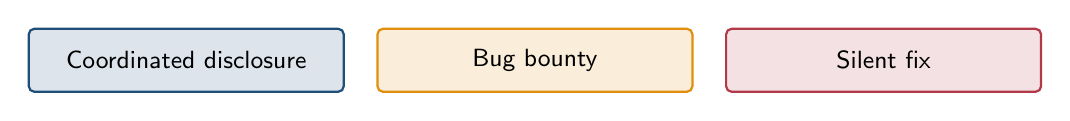
\begin{tikzpicture}[node distance=4mm]
  \node[isbox, fill=isOT!15, draw=isOT, minimum width=40mm, font=\small] (a) {Coordinated disclosure};
  \node[isbox, fill=isAccent!15, draw=isAccent, minimum width=40mm, font=\small, right=of a] (b) {Bug bounty};
  \node[isbox, fill=isAttack!15, draw=isAttack, minimum width=40mm, font=\small, right=of b] (c) {Silent fix};
\end{tikzpicture}
\vspace{2mm}
\begin{notebox}{Why ICS lags}
Vendor patch cycles average \textbf{90--180 days}; many critical CVEs are released without code. Always check the security advisory page weekly, not the homepage.
\end{notebox}
\note{
  Coordinated disclosure is the gold standard: researcher reports privately, vendor patches, advisory drops together --- this is how Siemens ProductCERT and Rockwell PSIRT operate. Bug bounties are still rare in OT but Schneider Electric and ABB have programmes worth knowing about. The ugly category is silent fix --- a vendor patches a bug in a firmware changelog entry that reads ``stability improvements''; this happens more than the industry admits. War story: a major drive vendor took 18 months between researcher report and shipping firmware for a critical RCE, because every customer in three regulated industries needed to schedule a maintenance window. Tell students to bookmark the security advisory subpages of the vendors they actually use, and to set RSS or email alerts --- the homepage will never tell them.
}
\end{frame}

\begin{frame}{Common ICS Weakness Patterns}
\begin{itemize}
  \item \textbf{CWE-798} -- hard-coded credentials in firmware
  \item \textbf{CWE-22}  -- path traversal in web UIs
  \item \textbf{CWE-787} -- out-of-bounds write in protocol parsers
  \item \textbf{CWE-306} -- missing authentication on critical functions
  \item \textbf{CWE-352} -- CSRF in HMI web interfaces
  \item \textbf{CWE-918} -- SSRF in cloud connectors
\end{itemize}
\begin{tipbox}{Pattern recognition}
Once you have read 50 ICS advisories you will start to recognise the same weaknesses across vendors.
\end{tipbox}
\source{MITRE, \emph{Common Weakness Enumeration} (CWE), \url{https://cwe.mitre.org}.}
\note{
  These six CWEs cover the majority of ICS advisories from the last five years --- Claroty's Team82 half-yearly reports back this up. Hard-coded credentials (CWE-798) are the embarrassment that keeps repeating because of debug accounts left in shipping firmware. The protocol-parser bugs (CWE-787) are the dangerous ones --- a single malformed Modbus or EtherNet/IP packet crashing the stack means anyone on the cell network can DoS a controller. Push back on the ``we have antivirus'' reflex: antivirus on the engineering workstation does nothing for a buffer overflow in the PLC's TCP stack itself, because the PLC has no agent and no patch until the vendor ships firmware. Encourage students to read raw advisories in the lab --- pattern recognition is the only way to triage 50 new CVEs a week.
}
\end{frame}

\begin{frame}{Honeypots and Deception}
\centering
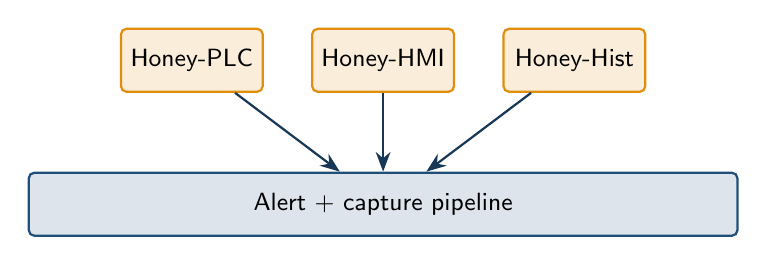
\begin{tikzpicture}[node distance=6mm]
  \node[plc, fill=isAccent!15, draw=isAccent] (h1) {Honey-PLC};
  \node[hmi, fill=isAccent!15, draw=isAccent, right=of h1] (h2) {Honey-HMI};
  \node[server, fill=isAccent!15, draw=isAccent, right=of h2] (h3) {Honey-Hist};
  \node[isbox, fill=isOT!15, draw=isOT, font=\small, below=10mm of h2, minimum width=90mm] (sink) {Alert + capture pipeline};
  \foreach \n in {h1,h2,h3}{\draw[flow] (\n) -- (sink);}
\end{tikzpicture}
\vspace{2mm}
\begin{notebox}{Examples}
\texttt{conpot} (open-source), GasPot, Cymmetria; sector-tailored ICS honeypots from MITRE Caldera and Dragos.
\end{notebox}
\note{
  Honeypots in OT are useful as an \emph{intelligence} tool, not a defence: any traffic hitting a fake Honey-PLC inside the cell network is by definition unwanted and worth alerting on. The catch is realism --- \texttt{conpot} fools casual Shodan crawlers but not a targeted attacker who tries to read a real-looking ladder programme. Stress the alert pipeline at the bottom of the diagram: without immediate routing into the SOC, a honeypot is just a logfile nobody reads. Real-world note: a sector-CERT in Europe runs a federated honeypot grid that has caught early stages of ransomware-affiliate scanning weeks before any victim went public. Briefly mention deception platforms like Acalvio and Illusive that go beyond a single fake host.
}
\end{frame}

\begin{frame}{Asset Criticality Classification}
\centering
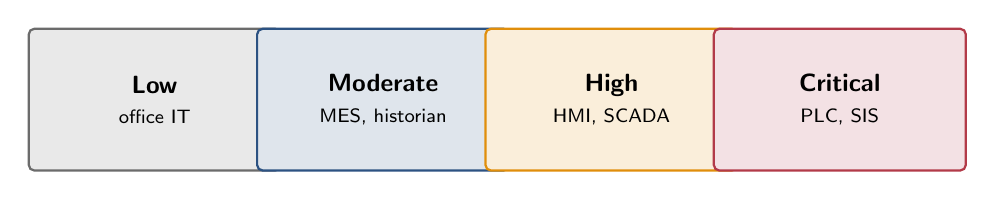
\begin{tikzpicture}[x=2.9cm]
  \node[isbox, fill=isMute!15, draw=isMute, minimum width=32mm, minimum height=18mm, align=center, font=\small] at (0,0) {\textbf{Low}\\\scriptsize office IT};
  \node[isbox, fill=isPLC!15, draw=isPLC, minimum width=32mm, minimum height=18mm, align=center, font=\small] at (1,0) {\textbf{Moderate}\\\scriptsize MES, historian};
  \node[isbox, fill=isAccent!15, draw=isAccent, minimum width=32mm, minimum height=18mm, align=center, font=\small] at (2,0) {\textbf{High}\\\scriptsize HMI, SCADA};
  \node[isbox, fill=isAttack!15, draw=isAttack, minimum width=32mm, minimum height=18mm, align=center, font=\small] at (3,0) {\textbf{Critical}\\\scriptsize PLC, SIS};
\end{tikzpicture}
\vspace{2mm}
\begin{notebox}{Drives priority}
The classification determines patch SLA, monitoring depth, and acceptable downtime.
\end{notebox}
\note{
  Classification is the lever that turns an asset inventory into a risk-managed programme --- without it, every CVE looks equally urgent and the team burns out. Walk through the four tiers and note that SIS (safety instrumented systems) live in their own world: any change requires functional-safety re-validation under IEC 61511, often months of work. Stress that the boundary between High and Critical is where most plant arguments happen --- operators want to call everything critical, security wants tighter scope. The classification also feeds the patch cadence table on the next slide: critical assets get the longest lead time, not the shortest, because the safety re-validation cost dominates. Encourage TAs to ask students which tier they would put a wireless field gateway in --- the answer depends entirely on what it controls.
}
\end{frame}

\begin{frame}{Patching Cadence -- IT vs OT}
\centering
\renewcommand{\arraystretch}{1.3}
\footnotesize
\begin{tabular}{|p{3.5cm}|p{4cm}|p{4cm}|}
\hline
\rowcolor{slidePanel}
 & \textbf{IT} & \textbf{OT} \\
\hline
Critical CVE        & 48--72 hours          & 30--90 days, with vendor approval \\
Normal patch        & Monthly Patch Tuesday & Annual maintenance window \\
Reboot tolerance    & Routine               & Co-ordinated, with operators \\
Rollback plan       & Standard              & Mandatory + tested \\
\hline
\end{tabular}
\vspace{2mm}
\begin{importantbox}{Compensating controls}
When you cannot patch quickly, deploy a virtual patch (IPS rule) or tighten the firewall around the affected service.
\end{importantbox}
\note{
  The right-hand column is the single biggest culture shock for students coming from IT. Patch Tuesday does not exist in OT --- a ``critical'' patch may take 30 to 90 days simply because the vendor requires regression testing on the customer's exact firmware band before authorising deployment. The mandatory rollback row is not optional: if a patched controller refuses to come back up, a half-staffed Sunday night shift cannot improvise. War story to land: a refinery sat on a critical EtherNet/IP CVE for 18 months because the annual turnaround was the only opportunity to take the affected cell offline --- they bridged the gap with a Tofino IPS rule that dropped the malformed packet upstream. That virtual patch was the only thing standing between them and CVE exposure for a year and a half.
}
\end{frame}

\begin{frame}{Summary -- Section \sectionNumber}
\begin{takeawaybox}{What to remember from this section}
\begin{itemize}\setlength{\itemsep}{2pt}
  \item Track CVEs from CISA, vendor PSIRTs, and threat intel feeds.
  \item Asset inventory with firmware versions is the foundation.
  \item CVSS base alone misleads -- always add environmental and process impact.
  \item Active scans only on test benches; passive sniffing is the production-safe default.
\end{itemize}
\end{takeawaybox}
\note{
  Recap the four pillars: feeds, inventory, environmental scoring, and scanning hygiene --- if students forget everything else, these four keep them from making the worst mistakes. Re-emphasise that the OT vulnerability programme is measured in months and years, not hours and days, and that compensating controls are a first-class deliverable, not a failure mode. Tease the next section: with vulnerabilities catalogued and prioritised, the natural next question is how attackers chain them into incidents --- which is the threat-modelling and attack-path material. Optional closing question for the room: ``Name one thing you will do differently when you read your next CVE advisory.'' Their answers tell the TA whether the environmental-modifier message landed.
}
\end{frame}

\referencesframe{
  \item FIRST. \emph{Common Vulnerability Scoring System v3.1 Specification Document}, 2019.
  \item MITRE. \emph{Common Weakness Enumeration (CWE)}, \url{https://cwe.mitre.org}.
  \item CISA. \emph{ICS Advisories archive}, \url{https://www.cisa.gov/news-events/cybersecurity-advisories/ics-advisories}.
  \item NIST. \emph{National Vulnerability Database (NVD)}, \url{https://nvd.nist.gov}.
  \item Forescout Vedere Labs. ICS vulnerability research (e.g.\ Ripple20, Urgent/11, Project Memoria).
  \item Claroty Team82. \emph{ICS Risk \& Vulnerability Reports}, half-yearly.
  \item Dragos. \emph{Year in Review}, annual.
  \item Stouffer, K. et al. \emph{NIST SP 800-82 Rev.\,3}, Sep 2023 (vulnerability management for OT).
  \item Bytes Lab et al. \emph{CodeSys CoDe16 advisories}, 2023.
  \item INL. \emph{Recommended Practice: Patch Management for Control Systems}, 2008.
}

\closingframe

\end{document}
